\documentclass[10pt,aspectratio=169]{beamer}

\usetheme[progressbar=frametitle]{metropolis}

% remove indentation throughout the document
\setlength{\parindent}{0pt}

\usepackage{tocbasic}

%%% Doc: ftp://tug.ctan.org/pub/tex-archive/macros/latex/contrib/caption/caption.pdf
\usepackage[tableposition=above]{caption}

% Aussehen der Captions
\captionsetup{
   margin = 10pt,
   font = {rm},
   labelfont = {bf},
   format = plain, % oder 'hang'
   indention = 0em,  % Einruecken der Beschriftung
   labelsep = space, %period, space, quad, newline
   justification = RaggedRight, % justified, centering, RaggedRight
   singlelinecheck = true, % false (true=bei einer Zeile immer zentrieren)
   position = bottom %top
}

%%% Bugfix Workaround
\DeclareCaptionOption{parskip}[]{}
\DeclareCaptionOption{parindent}[]{}

\usepackage{csquotes}
\usepackage{siunitx}

%% useful abreviations

\newcommand\ie{i.\,e.\xspace}
\newcommand\eg{e.\,g.\xspace}
\newcommand\Eg{E.\,g.\xspace}
\newcommand\NB{N.\,B.\xspace}
\newcommand\BSc{B.\,Sc.\xspace}
\newcommand\MSc{M.\,Sc.\xspace}
\newcommand\PhD{Ph.\,D.\xspace}
\newcommand\etc{etc.\xspace}
\newcommand\cf{cf.\xspace}
\newcommand\Cf{Cf.\xspace}
\newcommand\etal{et\,al.\xspace}
\newcommand\page[1]{p.\,#1}
\newcommand\pages[1]{pp.\,#1}
\newcommand\ham{a.\,m.\xspace}
\newcommand\hpm{p.\,m.\xspace}
	
\newcommand\zB{z.\,B.\xspace}
\newcommand\proz{\,\%\xspace}

%% Useful definitions for tables --------------------------------------------------------- %% 

% um Tabellenspalten mit Flattersatz zu setzen, muss \\ vor
% (z.B.) \raggedright geschuetzt werden:
\newcommand{\PreserveBackslash}[1]{\let\temp=\\#1\let\\=\temp}

% Linksbuendig:
\newcolumntype{v}[1]{>{\PreserveBackslash\RaggedRight\hspace{0pt}}p{#1}}
\newcolumntype{M}[1]{>{\PreserveBackslash\RaggedRight\hspace{0pt}}m{#1}}
\newcolumntype{Y}{>{\PreserveBackslash\RaggedLeft\hspace{0pt}}X}
%%% Spalten fuer Mathematik
%
% serifenlose Matheschrift
%\newcolumntype{s}[1]{%
%  >{\DC@{.}{,}{#1}\mathsf\bgroup}l%
%  <{\egroup\DV@end}%
%}

% Tabellenspaltentyp fuer den Kopf: (Farbe + Ausrichtung)
\newcolumntype{H}[1]{>{\columncolor{tableheadcolor}}l}

%%% ---|Layout der Tabellen |-------------------

% Neue Umgebung fuer Tabellen:

\newenvironment{Tabelle}[2][c]{%
  \tablestylecommon
  \begin{longtable}[#1]{#2}
  }
  {\end{longtable}%
  \tablerestoresettings
}

% Groesse der Schrift in Tabellen
\newcommand{\tablefontsize}{ \footnotesize}
\newcommand{\tableheadfontsize}{\footnotesize}

% Layout der Tabelle: Ausrichtung, Schrift, Zeilenabstand
\newcommand\tablestylecommon{%
  \renewcommand{\arraystretch}{1.4} % Groessere Abstaende zwischen Zeilen
  \normalfont\normalsize            %
  \sffamily\tablefontsize           % Serifenlose und kleine Schrift
  \centering%                       % Tabelle zentrieren
}

\newcommand{\tablestyle}{
  \tablestylecommon
  %\tablealtcolored
}

% Ruecksetzten der Aenderungen
\newcommand\tablerestoresettings{%
  \renewcommand{\arraystretch}{1}% Abstaende wieder zuruecksetzen
  \normalsize\rmfamily % Schrift wieder zuruecksetzen
}

% Tabellenkopf: Serifenlos+fett+schraeg+Schriftfarbe
\newcommand\tableheads{%
  \tableheadfontsize%
  \sffamily\bfseries%
  %\slshape
  %\color{white}
}

\newcommand\tablesubheadfont{%
  \tableheadfontsize%
  \sffamily\bfseries%
  \slshape
  %\color{white}
}

\newcommand\tableheadcolor{%
  %\rowcolor{tablesubheadcolor}
  %\rowcolor{tableblackheadcolor}
  \rowcolor{tableheadcolor}%
}

\newcommand\tablesubheadcolor{%
  \rowcolor{tablesubheadcolor}
  %\rowcolor{tableblackheadcolor}
}

\newcommand{\tableend}{\arrayrulecolor{black}\hline}

% Tabellenkopf (1=Spaltentyp, 2=Text)
% \newcommand{\tablehead}[2]{
%   \multicolumn{1}{#1@{}}{%
%     \raisebox{.1mm}{% Ausrichtung der Beschriftung
%       #2%
%     }\rule{0pt}{4mm}}% unsichtbare Linie, die die Kopfzeile hoeher macht
% }


\newcommand{\tablesubhead}[2]{%
  \multicolumn{#1}{>{\columncolor{tablesubheadcolor}}l}{\tablesubheadfont #2}%
}

% Tabellenbody (=Inhalt)
\newcommand\tablebody{%
\tablefontsize\sffamily\upshape%
}

\newcommand\tableheadshaded{%
  \rowcolor{tableheadcolor}%
}
\newcommand\tablealtcolored{%
  \rowcolors{1}{tablerowcolor}{white!100}%
}
%%% --------------------------------------------

\usepackage{ragged2e}

%% Rotate table head
%% http://tex.stackexchange.com/questions/98388/how-to-make-table-with-rotated-table-headers-in-latex
%% http://tex.stackexchange.com/questions/32683/rotated-column-titles-in-tabular
\newcommand*\rottblhead{\rotatebox{75}}

\usepackage{cleveref}

\newcommand\stress[1]{{\color{red}#1}} 

% \mathds{1}
\usepackage{dsfont}

\usepackage{tabularx}

\usepackage{siunitx}
\DeclareSIUnit\barsi{\text{bar}}

\usepackage{subfig}

\usepackage{tikz}
\usetikzlibrary{shapes}
\usetikzlibrary{plotmarks}
\usetikzlibrary{fit}
\usetikzlibrary{overlay-beamer-styles}
\usetikzlibrary{positioning}
\usetikzlibrary{calc}
\usetikzlibrary{decorations.pathreplacing}
\usetikzlibrary{decorations.pathmorphing}
\definecolor{lightblue}{RGB}{189,216,238}

\usepackage{etoolbox}

\title{Non-Parametric Machine Learning Models for Solar Energy Forecasting}
% \subtitle{}
\date{16.07.2021}
\author{Pavel Zwerschke}
\institute{Karlsruhe Institute of Technology}
\titlegraphic{\hfill\includegraphics[height=1.5cm]{logos/kitlogo_en_cmyk}}

\usepackage[style=authoryear, maxcitenames=2, bibencoding=inputenc]{biblatex}
\bibliography{bibliography.bib}

\begin{document}

\maketitle

\begin{frame}{Table of contents}
    \setbeamertemplate{section in toc}[sections numbered]
    \tableofcontents%[hideallsubsections]
\end{frame}

\begin{frame}{Introduction}
    \begin{itemize}
        \item Solar energy generation is characterized by fluctuations due to uncertainty of the weather
        \item Uncertainty should be quantified through a probabilistic forecast
        \begin{itemize}
            \item Probabilistic forecasts for solar energy generation are underdeveloped
            \item[\(\leadsto\)] We want to compare different machine learning based forecasting models on solar power
        \end{itemize}
    \end{itemize}
\end{frame}

\section{Model descriptions}

\begin{frame}{NNQF [\cite{Ordiano2020}]}
    \begin{center}
        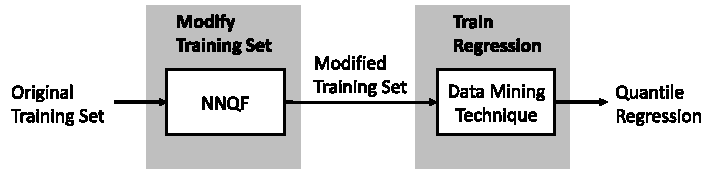
\includegraphics{plots/nnqf_approach.pdf}
    \end{center}
    \begin{itemize}
        \item Let \(x_1, \ldots, x_n \in \R^D\) be the predictors and \(y_1, \ldots, y_n\in \R\) the target values.
        \item Calculate approximate quantiles of \(y_i\):
        \begin{itemize}
            \item Find \(N\) nearest neighbors of \(x_i\): \(\set{x_{i_1}, \ldots, x_{i_N}}\)
            \item Calculate the empirical quantiles \(y_{(0.01)}, \ldots, y_{(0.99)}\) from \(\set{y_{i_1}, \ldots, y_{i_N}}\)
        \end{itemize}
    \end{itemize}
\end{frame}

\begin{frame}{NNQF [\cite{Ordiano2020}]}
    \begin{itemize}
        \item After modification of training set, a data mining technique is used for learning the map \(f(x) = (y_{(0.01)}, \ldots, y_{(0.99)})\).
        \item High correlation of adjacent data points
        \begin{itemize}
            \item[\(\leadsto\)] use lag features: don't just use \(x_i\) for prediction of \(y_i\), but also 
            \(x_{i-1}, \ldots, x_{i-H+1}\)
            \item regression model now predicts \( \P(y_i | x_i, \ldots, x_{i-H+1}) \)
        \end{itemize}
    \end{itemize}
\end{frame}

\begin{frame}{Advantages of NNQF [\cite{Ordiano2020}]}
    \begin{itemize}
        \item the regression technique is not specified, any technique can be used
        \begin{itemize}
            \item in the classical quantile regression techniques and QRF, the algorithm needs to be specified
        \end{itemize}
        \item nearest neighbor calculation only needs to be done once
        \begin{itemize}
            \item nearest neighbor quantile regression calculates the nearest neighbors for each prediction
        \end{itemize}
        \item the original dataset does not need to be saved
    \end{itemize}
\end{frame}

\begin{frame}{QRF [\cite{Meinshausen2006}]}
    \begin{itemize}
        \item Use bagging to produce \(k\) trees from training set \(x_1, \ldots, x_n \in \R^D\) and \(y_1, \ldots, y_n \in \R\)
        \item For \(x\in \R^D\), we want to predict the distribution \(\P(Y | X=x)\)
        \begin{itemize}
            \item Calculate \(\hat{y}_1, \ldots, \hat{y}_k\) from the trees 
            \item Calculate the empirical quantiles \(\hat{y}_{(q)}\) of \(\set{\hat{y}_1, \ldots, \hat{y}_k}\) for any \(q \in (0,1)\)
        \end{itemize}
    \end{itemize}
\end{frame}

\begin{frame}[fragile]{DeepAR -- Training [\cite{Salinas2020}]}
    \begin{center}
        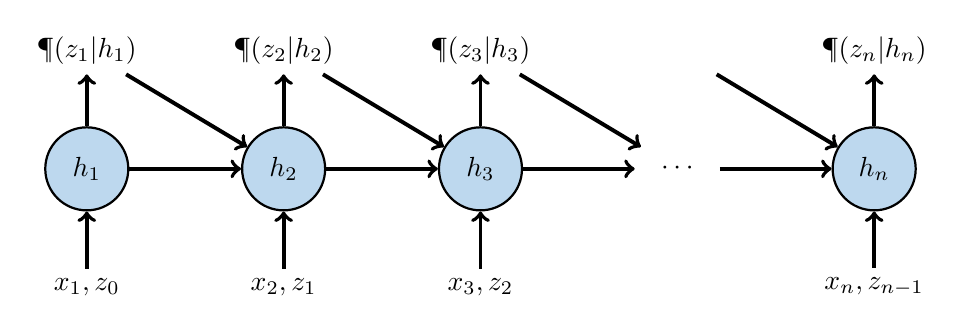
\begin{tikzpicture}[yscale=-1,node distance=-\pgflinewidth]
    \tikzset{ReceptorNode/.style={circle, draw=black, fill=lightblue, thick, inner sep=2pt, minimum size=30pt}}
    \tikzset{Placeholder/.style={circle, thick, inner sep=2pt, minimum size=30pt}}
    \tikzset{Connection/.style={->, line width=0.5mm}}
    \newcommand{\mynode}[3]{
        \node[ReceptorNode] (circ-#2) at (#1, 0) {\(\boldsymbol{h}_{#2}\)};
        \node (x-#2) at (#1, 1.5) {\(x_{#2}, z_{#3}\)};
        \node (y-#2) at (#1, -1.5) {\(\P(z_{#2}|\boldsymbol{h}_{#2})\)};

        \draw[Connection] (circ-#2) -- (y-#2);
        \draw[Connection] (x-#2)    -- (circ-#2);
    }
    \newcommand{\placeholder}[2]{
        \node[Placeholder] (circ-#2) at (#1, 0) {\(\cdots\)};
        \node (x-#2) at (#1, 1.5) {};
        \node[opacity=0] (y-#2) at (#1, -1.5) {\(\P(z_{#2}|\boldsymbol{h}_{#2})\)};
    }
    \newcommand{\connect}[2]{
        \draw[Connection] (y-#1)    -- (circ-#2);
        \draw[Connection] (circ-#1) -- (circ-#2);
    }

    % Create nodes
    \mynode{1 * 2.5}{1}{0}
    \mynode{2 * 2.5}{2}{1}
    \connect{1}{2}
    \mynode{3 * 2.5}{3}{2}
    \connect{2}{3}
    \placeholder{4 * 2.5}{4}
    \connect{3}{4}
    % Last node is called "n"
    \mynode{5*2.5}{n}{n-1}
    \connect{4}{n}
\end{tikzpicture}
    \end{center}
    \begin{itemize}
        \item Autoregressive Recurrent Neural Network with probabilistic output
        \item \(x_t\) and \(z_{t-1}\) form with \(\boldsymbol{h}_{t-1}\) the new network output \(\boldsymbol{h}_t\)
        which is used to compute the likelihood \(\P(z_t | \boldsymbol{h}_t)\)
    \end{itemize}
\end{frame}

\begin{frame}[fragile]{DeepAR -- Predicting [\cite{Salinas2020}]}
    \begin{center}
        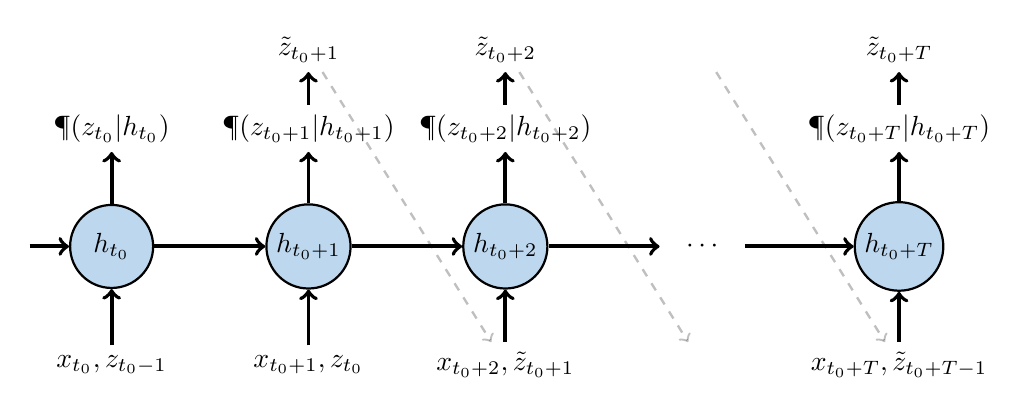
\begin{tikzpicture}[yscale=-1,node distance=-\pgflinewidth]
    \tikzset{ReceptorNode/.style={circle, draw=black, fill=lightblue, thick, inner sep=2pt, minimum size=30pt}}
    \tikzset{Placeholder/.style={circle, thick, inner sep=2pt, minimum size=30pt}}
    \tikzset{Connection/.style={->, line width=0.5mm}}
    \tikzset{LightConnection/.style={->, dashed, line width=0.3mm, opacity=0.25}}
    \newcommand{\mynode}[3]{
        \node[ReceptorNode] (circ-#2) at (#1, 0) {\(\boldsymbol{h}_{#2}\)};
        \node (x-#2) at (#1, 1.5) {\(x_{#2}, z_{#3}\)};
        \node (y-#2) at (#1, -1.5) {\(\P(z_{#2}|\boldsymbol{h}_{#2})\)};

        \draw[Connection] (circ-#2) -- (y-#2);
        \draw[Connection] (x-#2)    -- (circ-#2);
    }
    \newcommand{\mynodewithresult}[3]{
        \node[ReceptorNode] (circ-#2) at (#1, 0) {\(\boldsymbol{h}_{#2}\)};
        \node (x-#2) at (#1, 1.5) {\(x_{#2}, z_{#3}\)};
        \node (y-#2) at (#1, -1.5) {\(\P(z_{#2}|\boldsymbol{h}_{#2})\)};
        \node (z-#2) at (#1, -2.5) {\(\tilde{z}_{#2}\)};

        \draw[Connection] (circ-#2) -- (y-#2);
        \draw[Connection] (x-#2)    -- (circ-#2);
        \draw[Connection] (y-#2)    -- (z-#2);
    }
    \newcommand{\mynodewithresultinputsampled}[3]{
        \node[ReceptorNode] (circ-#2) at (#1, 0) {\(\boldsymbol{h}_{#2}\)};
        \node (x-#2) at (#1, 1.5) {\(x_{#2}, \tilde{z}_{#3}\)};
        \node (y-#2) at (#1, -1.5) {\(\P(z_{#2}|\boldsymbol{h}_{#2})\)};
        \node (z-#2) at (#1, -2.5) {\(\tilde{z}_{#2}\)};

        \draw[Connection] (circ-#2) -- (y-#2);
        \draw[Connection] (x-#2)    -- (circ-#2);
        \draw[Connection] (y-#2)    -- (z-#2);
    }
    \newcommand{\placeholder}[2]{
        \node[Placeholder] (circ-#2) at (#1, 0) {\(\cdots\)};
        \node (x-#2) at (#1, 1.5) {\phantom{\(x_{#2}, \tilde{z}_{#2}\)}};
        \node (y-#2) at (#1, -1.5) {\phantom{\(\P(z_{#2}|h_{#2})\)}};
        \node (z-#2) at (#1, -2.5) {\phantom{\(\tilde{z}_{#2}\)}};
    }
    \newcommand{\connect}[2]{
        \draw[Connection] (circ-#1) -- (circ-#2);
    }
    \newcommand{\connectsampled}[2]{
        \draw[LightConnection] (z-#1) -- (x-#2);
        \draw[Connection] (circ-#1)   -- (circ-#2);
    }

    % Create nodes
    \mynode{1 * 2.5}{t_0}{t_0-1}
    \draw[Connection] ([xshift=-0.5cm]circ-t_0.west) -- (circ-t_0);
    \onslide<2->{
        \mynodewithresult{2 * 2.5}{t_0+1}{t_0}
        \connect{t_0}{t_0+1}
    }
    \onslide<3->{
        \mynodewithresultinputsampled{3 * 2.5}{t_0+2}{t_0+1}
        \connectsampled{t_0+1}{t_0+2}
    }
    \onslide<4->{
        \placeholder{4 * 2.5}{t_0+3}
        \connectsampled{t_0+2}{t_0+3}
    }
    % Last node is called "t_0+T"
    \onslide<5->{
        \mynodewithresultinputsampled{5*2.5}{t_0+T}{t_0+T-1}
        \connectsampled{t_0+3}{t_0+T}
    }
\end{tikzpicture}
    \end{center}
    \begin{itemize}
        \onslide<2->{\item Generate \(\tilde{z}_t \sim \P(\cdot | \boldsymbol{h}_t)\) and use it in the next step as input}
    \end{itemize}
\end{frame}

\begin{frame}{SQF-RNN [\cite{Gasthaus2019}]}
    \begin{columns}
    \begin{column}{0.6\textwidth}
    \begin{itemize}
        \item Main difference to DeepAR is output distribution
        \begin{itemize}
            \item Given by monotonously increasing linear splines: 
            \[ s(x; \gamma, b, d) = \gamma + \sum_{l=0}^L b_l (x - d_l)_+ \]
            \item Arbitrary distribution can be fit \(\leadsto\) no assumption on distribution
        \end{itemize}
    \end{itemize}
    \end{column}

    \begin{column}{0.35\textwidth}
        \begin{tikzpicture}[scale=0.6]
    \pgfplotsset{every axis/.style={mlineplot}}
    \begin{axis}[xmin=-0.05, xmax=1.05, ymin=-0.1, ymax=2.1]
        \addplot[domain = 0:1] {tanh(4*x-2)-tanh(-2)};
        \addplot[domain = 0:0.3] {x};
        \addplot[domain = 0.3:0.7] {0.3 + 3.3 * (x - 0.3)};
        \addplot[domain = 0.7:1] {1.62 + 1.02 * (x - 0.7)};
    \end{axis}
\end{tikzpicture}
    \end{column}
    \end{columns}
\end{frame}

\begin{frame}{Summary}
    \begin{itemize}
        \item NNQF
        \begin{itemize}
            \item Preprocessing with nearest neighbor filters \(\leadsto\) regression for preprocessed data
        \end{itemize}
        \item QRF
        \begin{itemize}
            \item Random Forests \(\leadsto\) take empirical quantiles of result
        \end{itemize}
        \item SQF-RNN
        \begin{itemize}
            \item Deep neural network with autoregressive input
            \item Target distribution modeled by spline quantile functions
        \end{itemize}
    \end{itemize}
\end{frame}

\begin{frame}{Plots}
    \begin{columns}
        \begin{column}{0.33\textwidth}
            \includegraphics[width=\textwidth]{plots/nnqf_plot_9.pdf}
            \begin{center}
                NNQF
            \end{center}
        \end{column}
        \begin{column}{0.33\textwidth}
            \includegraphics[width=\textwidth]{plots/qrf_plot_9.pdf}
            \begin{center}
                QRF
            \end{center}
        \end{column}
        \begin{column}{0.33\textwidth}
            \includegraphics[width=\textwidth]{plots/sqf_rnn_plot_9.pdf}
            \begin{center}
                SQF-RNN
            \end{center}
        \end{column}
    \end{columns}
\end{frame}

\section{Comparison}

\begin{frame}{Feature importance}
    \begin{center}
        \begin{tikzpicture}
    \begin{axis}[
        width  = \textwidth,
        height = 0.3\textheight,
        major x tick style = transparent,
        ybar,
        bar width=10pt,
        ymajorgrids = true,
        ylabel = {Feature importance},
        xtick = {1,2,3,4,5,6},
        xticklabel style={align=center},
        xticklabels = {Surface\\solar\\rad down, Surface\\thermal\\rad down, Top net\\solar rad, Total\\precipitation, Total\\cloud cover, Previous\\points},
        scaled y ticks = false,
    ]
        \addplot
            coordinates {(1, 1.3365) (2, 1.0214) (3, 1.0199) (4, 1.0020) (5, 1.0025)};
        \addplot
            coordinates {(1, 1.2202) (2, 1.0052) (3, 1.0856) (4, 1.0032) (5, 1.0405)};
        \addplot
            coordinates {(1, 1.0268) (2, 1.0208) (3, 1.0516) (4, 1.0124) (5, 1.2059) (6, 1.0918)};

        \legend{QRF, NNQF, SQF-RNN}
    \end{axis}
\end{tikzpicture}
    \end{center}
\end{frame}

\begin{frame}[fragile]{Pinball loss}
    \begin{columns}
    \begin{column}{0.5\textwidth}
        \begin{flushright}
            \begin{tikzpicture}[scale=0.6]
    \pgfplotsset{every axis/.style={mlineplot}}
    \begin{axis}[title=Pinball loss, 
                 xlabel=Month, 
                 ylabel=loss, 
                 xtick={4,6,8,10,12,14}, 
                 xticklabels={Jul, Sep, Nov, Jan, Mar, May}]
        % NNQF
        \addplot coordinates {(4, 0.01559) (5, 0.02091) (6, 0.01896) (7, 0.02267) (8, 0.02330) (9, 0.02334) (10, 0.02333) (11, 0.02038) (12, 0.01912) (13, 0.01673) (14, 0.01363) (15, 0.01480)};
        % QRF
        \addplot coordinates {(4, 0.01559) (5, 0.02100) (6, 0.01983) (7, 0.02350) (8, 0.02447) (9, 0.02370) (10, 0.02483) (11, 0.02160) (12, 0.01932) (13, 0.01694) (14, 0.01536) (15, 0.01526)};
        % SQF-RNN
        \addplot coordinates {(4, 0.02581) (5, 0.03041) (6, 0.02451) (7, 0.01895) (8, 0.01707) (9, 0.01833) (10, 0.02002) (11, 0.02104) (12, 0.02204) (13, 0.01684) (14, 0.01338) (15, 0.02041)};
        % DeepAR
        \addplot coordinates {(4, 0.02634) (5, 0.03649) (6, 0.02744) (7, 0.01958) (8, 0.02579) (9, 0.02290) (10, 0.02320) (11, 0.02612) (12, 0.02424) (13, 0.02282) (14, 0.01865) (15, 0.01889)};
        \legend{NNQF, QRF, SQF-RNN, DeepAR}
    \end{axis}
\end{tikzpicture}
        \end{flushright}
    \end{column}
    \begin{column}{0.5\textwidth}
        Mean losses:
        \begin{description}
            \item[\textcolor{TolDarkBlue}{NNQF}] \(0.01940\), place 16/24
            \item[\textcolor{TolLightBrown}{QRF}] \(0.02015\), place 17/24
            \item[\textcolor{TolLightGreen}{SQF-RNN}] \(0.02041\), place 18/24
            \item[\textcolor{TolDarkBrown}{DeepAR}] \(0.02437\), place 20/24
        \end{description}
    \end{column}
    \end{columns}
    
    \begin{itemize}
        \item NNQF and QRF perform very similar
        \item In the summer months (southern hemisphere!), SQF-RNN performs noticably better than NNQF and QRF models
        \begin{itemize}
            \item[\(\leadsto\)] NNQF and QRF only focus on solar radiation, not on total cloud cover
        \end{itemize}
    \end{itemize}
\end{frame}

\begin{frame}[fragile]{Energy score}
    \begin{columns}
    \begin{column}{0.5\textwidth}
    \begin{flushright}
        \section{Energy score}

The energy score is a proper scoring rule that is used for 
evaluating multi dimensional forecasts. A time series \((y_t)_t\) 
can be evaluated in this fashion by looking at a sequence of \(H\) 
points, i.e. \((y_t, \ldots, y_{t-H+1})_t \in \R^H\). 
The scoring rule is defined as follows:
\[ \mathrm{S}(P, y) = \mathbb{E}_P ||Y-y||_2 - \frac{1}{2} \mathbb{E}_P ||Y-Y'||_2, \]
where \(Y'\) is an i.i.d. copy of \(Y\), so it is drawn independently with the same distribution \(P\).

This scoring rule takes the time series attributes, namely the 
correlation of adjacent data points, into account while 
the pinball loss only evaluates the score pointwise.

The results of the energy score are shown in Figure \ref{fig:energy-score}. 
We can observe that the SQF-RNN model performs better than or at least similar 
to the NNQF and QRF models in every month with July and August as exception. 
Another thing to note is that the DeepAR model always performs worse than the SQF-RNN model. 

\begin{figure}[ht]
    \centering
    \section{Energy score}

The energy score is a proper scoring rule that is used for 
evaluating multi dimensional forecasts. A time series \((y_t)_t\) 
can be evaluated in this fashion by looking at a sequence of \(H\) 
points, i.e. \((y_t, \ldots, y_{t-H+1})_t \in \R^H\). 
The scoring rule is defined as follows:
\[ \mathrm{S}(P, y) = \mathbb{E}_P ||Y-y||_2 - \frac{1}{2} \mathbb{E}_P ||Y-Y'||_2, \]
where \(Y'\) is an i.i.d. copy of \(Y\), so it is drawn independently with the same distribution \(P\).

This scoring rule takes the time series attributes, namely the 
correlation of adjacent data points, into account while 
the pinball loss only evaluates the score pointwise.

The results of the energy score are shown in Figure \ref{fig:energy-score}. 
We can observe that the SQF-RNN model performs better than or at least similar 
to the NNQF and QRF models in every month with July and August as exception. 
Another thing to note is that the DeepAR model always performs worse than the SQF-RNN model. 

\begin{figure}[ht]
    \centering
    \section{Energy score}

The energy score is a proper scoring rule that is used for 
evaluating multi dimensional forecasts. A time series \((y_t)_t\) 
can be evaluated in this fashion by looking at a sequence of \(H\) 
points, i.e. \((y_t, \ldots, y_{t-H+1})_t \in \R^H\). 
The scoring rule is defined as follows:
\[ \mathrm{S}(P, y) = \mathbb{E}_P ||Y-y||_2 - \frac{1}{2} \mathbb{E}_P ||Y-Y'||_2, \]
where \(Y'\) is an i.i.d. copy of \(Y\), so it is drawn independently with the same distribution \(P\).

This scoring rule takes the time series attributes, namely the 
correlation of adjacent data points, into account while 
the pinball loss only evaluates the score pointwise.

The results of the energy score are shown in Figure \ref{fig:energy-score}. 
We can observe that the SQF-RNN model performs better than or at least similar 
to the NNQF and QRF models in every month with July and August as exception. 
Another thing to note is that the DeepAR model always performs worse than the SQF-RNN model. 

\begin{figure}[ht]
    \centering
    \input{plots/energy_score}
    \caption[Energy score]{Energy score. 
    This graph plots the scores of the models for each month of the dataset competition. A lower score means a better performance.}
    \label{fig:energy-score}
\end{figure}

QRF returns a mean score of \(0.36759\), NNQF a mean score of \(0.36736\), 
SQF-RNN a mean score of \(0.36644\) and DeepAR a mean score of \(0.44235\).
    \caption[Energy score]{Energy score. 
    This graph plots the scores of the models for each month of the dataset competition. A lower score means a better performance.}
    \label{fig:energy-score}
\end{figure}

QRF returns a mean score of \(0.36759\), NNQF a mean score of \(0.36736\), 
SQF-RNN a mean score of \(0.36644\) and DeepAR a mean score of \(0.44235\).
    \caption[Energy score]{Energy score. 
    This graph plots the scores of the models for each month of the dataset competition. A lower score means a better performance.}
    \label{fig:energy-score}
\end{figure}

QRF returns a mean score of \(0.36759\), NNQF a mean score of \(0.36736\), 
SQF-RNN a mean score of \(0.36644\) and DeepAR a mean score of \(0.44235\).
    \end{flushright}
    \end{column}
    \begin{column}{0.5\textwidth}
    Mean losses:
    \begin{description}
        \item[\textcolor{TolDarkBlue}{NNQF}] \(0.36736\)
        \item[\textcolor{TolLightBrown}{QRF}] \(0.36759\)
        \item[\textcolor{TolLightGreen}{SQF-RNN}] \(0.36644\)
        \item[\textcolor{TolDarkBrown}{DeepAR}] \(0.44235\)
    \end{description}
    \end{column}
    \end{columns}
    
    \begin{itemize}
        \item SQF-RNN \(\succ\) NNQF \(\approx\) QRF in the energy score
        \begin{itemize}
            \item Energy score takes time series attributes into account, SQF-RNN is better at that due to the RNN structure
        \end{itemize}
    \end{itemize}
\end{frame}

\section{Conclusion}

\begin{frame}{Conclusion}
    \begin{itemize}
        \item NNQF is best on average
        \item NNQF is slightly better than QRF
        \item SQF-RNN is noticably better in the months October till Febuary (summer)
        \item SQF-RNN is not really fit for this kind of problem, usually uses way more different correlated tracks
        \item SQF-RNN always outperforms DeepAR (assumes Student's \(t\)-distribution)
        \begin{itemize}
            \item[\(\leadsto\)] SQF-RNN better suited for nonparametric tasks like weather forecasting
        \end{itemize}
    \end{itemize}
\end{frame}

\begin{frame}{References}
    \printbibliography[heading=none]
\end{frame}

\end{document}